\documentclass{beamer}

\usetheme{anthem}
\usepackage{inconsolata}
\usepackage[scale=.9]{FiraSans}

\title{The \emph{anthem} presentation theme}
\author{Andreas Hinterreiter}
\date{\today}
\titlegraphic{
\includegraphics[height=1cm]{logo}}

\begin{document}

\begin{frame}[plain]
	\titlepage
\end{frame}

\section{A Section with a Figure}

\begin{frame}[plain]
\sectionfigure{
\includegraphics[width=.75\textwidth]{section}}
\sectionpage
\end{frame}

\begin{frame}{An ordinary frame}
\begin{columns}
\column{.5\textwidth}
	\begin{itemize}
		\item An item inside an \texttt{itemize} environment.
		\item Another item.
		\begin{itemize}
			\item A Subitem.
			\item Another, slightly longer subitem.
		\end{itemize}
		\item And, at last, a final item.
	\end{itemize}
\column{.5\textwidth}
	\begin{fancyblock}{A fancy block}
	\raggedright This is the \texttt{fancyblock} environment provided by \emph{anthem}.  It can be customized with \emph{mdframed} options (as seen below).
	\end{fancyblock}
\end{columns}
\end{frame}

\begin{frame}[plain]
\sectionfigure{
\includegraphics[width=.75\textwidth]{section}}
\specialsectionpage{Intermezzo}{A Special Section with a Figure}
\end{frame}

\begin{frame}{About the Special Sections}
\begin{itemize}
	\item If you want to have a section title page with some other addition to the section title than the default "Part ..." (such as e.g.~"Aside" or "Intermezzo"), you can use the \texttt{\textbackslash{}specialsectionpage\{addition\}\{title\}} command.
	\item You should not declare this "special section" with \texttt{\textbackslash{}section}, otherwise the \alert{numering might not be correct}.
	\item Unfortunately this means, that the special section will not show up in your PDF reader's table of content. I hope I can soon implement this feature in a much nicer way.
\end{itemize}
\end{frame}


\section*{An Ordinary Section}

\begin{frame}[plain]
\sectionpage
\end{frame}

\begin{frame}{Another frame}
\begin{columns}
\column{.6\textwidth}
	\begin{enumerate}
		\item An item inside an \texttt{itemize} environment.
		\item Another item.
		\begin{enumerate}
			\item A Subitem.
			\item Another, slightly longer subitem.
		\end{enumerate}
		\item And, at last, a final item.
	\end{enumerate}
\column{.4\textwidth}
	\begin{fancyblock}[
	innertopmargin=0pt,
	innerbottommargin=0pt,
	innerleftmargin=0pt,
	innerrightmargin=0pt]{A fancy figure}
		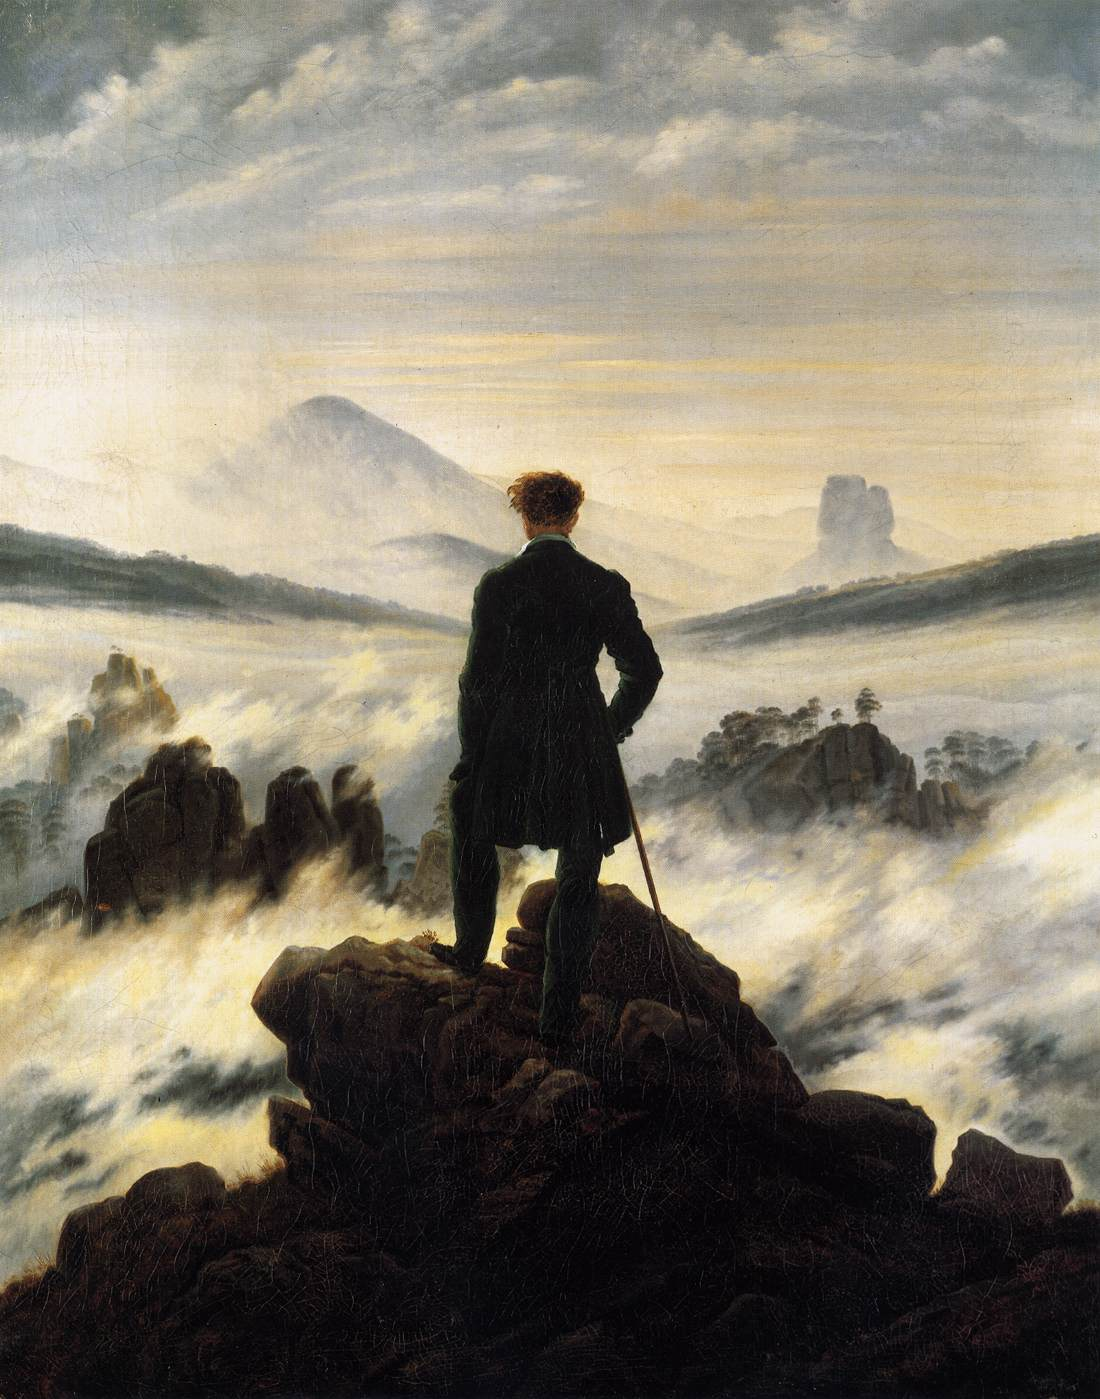
\includegraphics[width=\textwidth]{wanderer}
	\end{fancyblock}
\end{columns}
\end{frame}





\end{document}